\documentclass[12pt]{book}

\usepackage{natbib} % Tidies up citation numbers.
\usepackage[utf8]{inputenc}
\usepackage{graphicx}
\usepackage{pythonhighlight}
\usepackage{listingsutf8}
\usepackage{float}

%\def\UrlBreaks{\do\/\do-}
\usepackage[T1]{fontenc}
\usepackage{url}
\usepackage{breakurl}

\usepackage{pdfpages}

\lstset{
  extendedchars=true,
  language=java,
  basicstyle=\tiny\ttfamily,
  showspaces=false,
  showstringspaces=false,
    literate=
     {É}{{\'E}}{1}%
      {Á}{{\'A}}{1}%
      {Ã}{{\~A}}{1}%
      {Â}{{\^A}}{1}%
      {À}{{\`A}}{1}%
      {Ç}{{\,C}}{1}%
      {Ó}{{\'O}}{1}%
      {Í}{{\'I}}{1}%
      {Õ}{{\~O}}{1}%
      {Ú}{{\'U}}{1}%
      {ú}{{\'u}}{1}%
      {é}{{\'e}}{1}%
      {á}{{\'a}}{1}%
      {ã}{{\~a}}{1}%
      {à}{{\`a}}{1}%
      {â}{{\^a}}{1}%
      {ç}{{\,c}}{1}%
      {ó}{{\'o}}{1}%
      {í}{{\'i}}{1}%
      {õ}{{\~o}}{1}%
}

\definecolor{gray}{rgb}{0.4,0.4,0.4}
\definecolor{darkblue}{rgb}{0.0,0.0,0.6}
\definecolor{cyan}{rgb}{0.0,0.6,0.6}

\lstdefinelanguage{XML}
{
 numbers=left,
 numberstyle=\tiny,
 stepnumber=1,
 numbersep=8pt,
 morestring=[b]",
 morestring=[s]{>}{<},
 morecomment=[s]{<?}{?>},
 stringstyle=\color{black},
 identifierstyle=\color{darkblue},
 keywordstyle=\color{cyan},
 morekeywords={xmlns,version,type}% list your attributes here
}

\colorlet{punct}{red!60!black}
\definecolor{background}{HTML}{EEEEEE}
\definecolor{delim}{RGB}{20,105,176}
\colorlet{numb}{magenta!60!black}

\lstdefinelanguage{json}{
    basicstyle=\tiny\ttfamily,
    numbers=left,
    numberstyle=\tiny,
    stepnumber=1,
    numbersep=8pt,
    showstringspaces=false,
    breaklines=true,
    frame=lines,
    backgroundcolor=\color{background},
    literate=
     *{É}{{\'E}}{1}%
      {Á}{{\'A}}{1}%
      {Ã}{{\~A}}{1}%
      {Â}{{\^A}}{1}%
      {À}{{\`A}}{1}%
      {Ç}{{\,C}}{1}%
      {Ó}{{\'O}}{1}%
      {Í}{{\'I}}{1}%
      {Õ}{{\~O}}{1}%
      {Ú}{{\'U}}{1}%
      {ú}{{\'u}}{1}%
      {é}{{\'e}}{1}%
      {á}{{\'a}}{1}%
      {ã}{{\~a}}{1}%
      {à}{{\`a}}{1}%
      {â}{{\^a}}{1}%
      {ç}{{\,c}}{1}%
      {ó}{{\'o}}{1}%
      {í}{{\'i}}{1}%
      {õ}{{\~o}}{1}%
     {0}{{{\color{numb}0}}}{1}
      {1}{{{\color{numb}1}}}{1}
      {2}{{{\color{numb}2}}}{1}
      {3}{{{\color{numb}3}}}{1}
      {4}{{{\color{numb}4}}}{1}
      {5}{{{\color{numb}5}}}{1}
      {6}{{{\color{numb}6}}}{1}
      {7}{{{\color{numb}7}}}{1}
      {8}{{{\color{numb}8}}}{1}
      {9}{{{\color{numb}9}}}{1}
      {:}{{{\color{punct}{:}}}}{1}
      {,}{{{\color{punct}{,}}}}{1}
      {\{}{{{\color{delim}{\{}}}}{1}
      {\}}{{{\color{delim}{\}}}}}{1}
      {[}{{{\color{delim}{[}}}}{1}
      {]}{{{\color{delim}{]}}}}{1},
}

\lstdefinelanguage{SPARQL}{
    basicstyle=\tiny\ttfamily,
    numbers=left,
    numberstyle=\tiny,
    stepnumber=1,
    numbersep=8pt,
    showstringspaces=false,
    breaklines=true,
    frame=lines,
    backgroundcolor=\color{background},
    literate=
     {É}{{\'E}}{1}%
      {Á}{{\'A}}{1}%
      {Ã}{{\~A}}{1}%
      {Â}{{\^A}}{1}%
      {À}{{\`A}}{1}%
      {Ç}{{\,C}}{1}%
      {Ó}{{\'O}}{1}%
      {Í}{{\'I}}{1}%
      {Õ}{{\~O}}{1}%
      {Ú}{{\'U}}{1}%
      {ú}{{\'u}}{1}%
      {é}{{\'e}}{1}%
      {á}{{\'a}}{1}%
      {ã}{{\~a}}{1}%
      {à}{{\`a}}{1}%
      {â}{{\^a}}{1}%
      {ç}{{\,c}}{1}%
      {ó}{{\'o}}{1}%
      {í}{{\'i}}{1}%
      {õ}{{\~o}}{1},%
  morekeywords={
    SELECT,CONSTRUCT,DESCRIBE,ASK,WHERE,FROM,NAMED,PREFIX,BASE,OPTIONAL,
    FILTER,GRAPH,LIMIT,OFFSET,SERVICE,UNION,EXISTS,NOT,BINDINGS,MINUS,a
  }
}

\lstdefinelanguage{overpassQL}{
    basicstyle=\tiny\ttfamily,
    numbers=left,
    numberstyle=\tiny,
    stepnumber=1,
    numbersep=8pt,
    showstringspaces=false,
    breaklines=true,
    frame=lines,
    backgroundcolor=\color{background}
}

\lstset{language=R,
    literate=
    {<-}{{$\gets$}}1%
     {É}{{\'E}}{1}%
      {Á}{{\'A}}{1}%
      {Ã}{{\~A}}{1}%
      {Â}{{\^A}}{1}%
      {À}{{\`A}}{1}%
      {Ç}{{\,C}}{1}%
      {Ó}{{\'O}}{1}%
      {Í}{{\'I}}{1}%
      {Õ}{{\~O}}{1}%
      {Ú}{{\'U}}{1}%
      {ú}{{\'u}}{1}%
      {é}{{\'e}}{1}%
      {á}{{\'a}}{1}%
      {ã}{{\~a}}{1}%
      {à}{{\`a}}{1}%
      {â}{{\^a}}{1}%
      {ç}{{\,c}}{1}%
      {ó}{{\'o}}{1}%
      {í}{{\'i}}{1}%
      {õ}{{\~o}}{1},%
    basicstyle=\tiny\ttfamily,
    stringstyle=\color{red},
    otherkeywords={0,1,2,3,4,5,6,7,8,9},
    morekeywords={TRUE,FALSE},
    deletekeywords={data,frame,length,as,character},
    keywordstyle=\color{blue},
    commentstyle=\color{red},
}

\usepackage[brazil]{babel}  
\usepackage{xcolor}
%xcolor v2.12 (2016/05/11)384  Colors by Name4.1  Base colors (always available)black blue brown cyan darkgray gray green lightgray lime magenta olive orange pink purple red teal violet white yellow

\usepackage[nopostdot]{glossaries}
\setglossarystyle{altlist}
\PassOptionsToPackage{hyphens}{url}
\usepackage [colorlinks = true,
            linkcolor = blue,
            urlcolor  = blue,
            citecolor = blue,
            anchorcolor = blue]{hyperref} 

% gerador de lero-lero
\usepackage{lipsum}

\usepackage{pdfpages}

\newenvironment{itquote}
{\begin{quote}\itshape}
{\end{quote}}

\usepackage[commentmarkup=todo]{changes}

\usepackage{datetime2}

\usepackage{booktabs}

\usepackage{caption}
\input{packages-estudantes}

% define cores personalizadas para o texto de cada autor
\usepackage
%[final]
{changes}
%\usepackage{changes}
%\url{https://ctan.org/pkg/changes}

\definechangesauthor[name={Jorge Henrique Cabral Fernandes}, color=orange]{jhcf} % git-user: jhcf

\definechangesauthor[name={Alexsander Correa de Oliveira}, color=black]{KvotheKS} % git-user: KvotheKS OK

\definechangesauthor[name={Allann Gois Hoffmann}, color=orange]{AllannH} % git-user: AllannH OK

\definechangesauthor[name={André Larrosa Chimpliganond}, color=orange]{andrelarrosacrypt} % git-user: andrelarrosacrypt OK

\definechangesauthor[name={André Cássio Barros de Souza}, color=green]{andreloff} % git-user: andreloff OK

\definechangesauthor[name={Bruno Sanguinetti Regadas de Barros}, color=blue]{Jaxiii} % git-user: Jaxiii OK

\definechangesauthor[name={Enzo Nunes Leal Sampaio}, color=orange]{enzodevs2000} % git-user: enzodevs2000 OK

\definechangesauthor[name={Felipe Gomes Paradas}, color=pink]{fparadas} % git-user: fparadas OK

\definechangesauthor[name={Lucas de Almeida Bandeira Macedo}, color=teal]{ABMHub} % git-user: ABMHub OK

\definechangesauthor[name={Fernanda Macedo de Sousa}, color=magenta]{fernandams} % git-user: fernandams Ok

\definechangesauthor[name={Gabriel dos Santos Martins}, color=green]{gsmartins96} %  git-user: gsmartins96 OK

\definechangesauthor[name={Gabriel Faustino Lima da Rocha}, color=gray]{Faustino27} %  git-user: Faustino27 OK

\definechangesauthor[name={Gabriel Martins de Almeida}, color=purple]{GMalme} %  git-user: GMalme OK

\definechangesauthor[name={Gabriel Rocha Fontenele}, color=pink]{ngsylar} % git-user: ngsylar OK

\definechangesauthor[name={Ítalo Eduardo Dias Frota}, color=pink]{titofrota} % git-user: titofrota OK

\definechangesauthor[name={João Antonio Desidério de Moraes}, color=teal]{joaoadm94} % git-user: joaoadm94 OK

\definechangesauthor[name={Ualiton Ventura da Silva}, color=orange]{uventura} % git-user: uventura OK

\definechangesauthor[name={Pedro de Torres Maschio}, color=orange]{pedro-maschio} % git-user: pedro-maschio OK

\definechangesauthor[name={Tong Zhou}, color=orange]{Tong00020} % git-user: Tong00020 Ok

\definechangesauthor[name={Gustavo Rodrigues dos Santos}, color=pink]{gutorsantos} % git-user: gutorsantos OK

\definechangesauthor[name={Gustavo Tomás de Paula}, color=green]{gustavo-tomas} % git-user: gustavo-tomas OK

\definechangesauthor[name={Gustavo Macedo de Carvalho}, color=purple]{GustavoMacCar} % git-user: GustavoMacCar OK

\definechangesauthor[name={Arthur da Silveira Couto}, color=purple]{CrimsonCrown} % git-user: CrimsonCrown OK?

\definechangesauthor[name={Vitor de Oliveira Araujo Araruna}, color=orange]{vitorararuna} % git-user: vitorararuna OK

\definechangesauthor[name={Rafael dos Santos Silva}, color=red]{rafaelsilva21} % git-user: rafaelsilva21 OK

\definechangesauthor[name={Marcus Vinicius Oliveira de Abrantes}, color=red]{MarcusABR} % git-user: MarcusABR OK

\definechangesauthor[name={Mateus de Paula Rodrigues}, color=cyan]{MoustacheGolem} % git-user: MoustacheGolem OK

\definechangesauthor[name={Leonardo Alves Riether}, color=blue]{LeoRiether} % git-user: LeoRiether OK

\definechangesauthor[name={Tatiana Franco Pereira}, color=cyan]{Tatianafp} % git-user: Tatianafp OK

\definechangesauthor[name={Vinícius Caixeta de Souza}, color=orange]{vinis-caixe} % git-user: vinis-caixe OK

\definechangesauthor[name={Conrado Nunes Barbosa Neto}, color=blue]{Conras21} % git-user: Conras21 OK

\definechangesauthor[name={Stefano Luppi Sposito}, color=pink]{KawaiiStheno} % git-user: KawaiiStheno OK

\definechangesauthor[name={João Pedro Felix de Almeida}, color=teal]{DYosplay} % git-user: DYosplay OK

\definechangesauthor[name={João Víctor Siqueira de Araujo}, color=red]{StrawHat972} % git-user: StrawHat972 OK

\definechangesauthor[name={Raylan da Silva Sales}, color=pink]{Rayxan} % git-user: Rayxan OK

\definechangesauthor[name={Guilherme Oliveira Loiola}, color=blue]{guioliunb} % git-user: guioliunb OK

\definechangesauthor[name={Paulo Alvim Alvarenga}, color=purple]{alvimpaulo} % git-user: alvimpaulo OK

\definechangesauthor[name={Léo Akira Abe Barros}, color=red]{leoakir} % git-user: leoakir OK

\definechangesauthor[name={Enzo Yoshio Niho}, color=purple]{enzoyoshio} % git-user: enzoyoshio OK

\definechangesauthor[name={Daniel Rodrigues Cardoso}, color=blue]{DanielrCardoso} % git-user: DanielrCardoso OK

\definechangesauthor[name={Fernando Ferreira Cordeiro}, color=blue]{FernandoCordeiro} % git-user: FernandoCordeiro OK

\definechangesauthor[name={Jônatas Gomes Barbosa da Silva}, color=cyan]{jonatas1n} % git-user: jonatas1n OK

\definechangesauthor[name={Lucas Gabriel de Oliveira Gurgel Fernandes}, color=black]{lggurgel} % git-user: lggurgel OK

\definechangesauthor[name={Bruno Esteves Dalla Costa Filho}, color=red]{brunoedcf} % git-user: brunoedcf OK

\definechangesauthor[name={Paulo Mauricio Costa Lopes}, color=red]{RequiemDosVivos} % git-user: RequiemDosVivos OK

\definechangesauthor[name ={Caio Bernardon Nascif Kaawi Massucato}, color=blue]{CaioMassucato} % git-user: CaioMassucato OK 

\makenoidxglossaries
\loadglsentries{1-Introducao/tarefas/1.1-Glossario/estudantes/main}
\setcounter{tocdepth}{5}
\setcounter{secnumdepth}{5}
\captionsetup[table]{name=Quadro}
\renewcommand{\lstlistingname}{Listagem de Código}

\newcommand{\dataset}{\textit{dataset}}
\newcommand{\query}{\textit{query}}
\newcommand{\githubusername}{\textless githubusername\textgreater}

\begin{document}

\chapter{Análise Bibliográfica sobre Computação Quântica, por Raylan da Silva Sales\label{chap:bibliometria:jhcf}}

\section{Planejamento do estudo}

O planejamento o  desenho do estudo deve descrever as motivações, questões de interesse, escopo, limitações e objetivos do trabalho.

O planejamento do estudo deve motivar o tema escolhido e o interesse do autor.

No caso do meu trabalho, as perguntas que o nortearam foram:
\begin{itemize}
    \item Qual a base de conhecimentos científicos produzida em torno do tema simulação multiagente voltada à compreensão de fenômenos sociais, com ênfase em métodos experimentais? 
    \item Como a simulação multiagente tem sido usada para compreender fenômenos sociais, com ênfase em métodos experimentais? 
    \item Quais os principais termos e conceitos ligados à frente de pesquisa no tema simulação multiagente de fenômenos sociais, com ênfase em métodos experimentais? 
    \item Qual a estrutura social da comunidade, se é que existe, que pesquisa sobre o tema simulação multiagente de fenômenos sociais, com ênfase em métodos experimentais?
\end{itemize}

Um termo que vem ganhando forma ao longo dos últimos anos é a "Computação Quântica". Quando usado para referenciar os avanços tecnológicos, esse termo se refere a ciência que elabora e estuda o desenvolvimento de produções tecnológicas relacionadas a softwares e algoritmos. 

A computação quântica transcende os limites do desenvolvimento tecnológico que haviam em tempos passados e possibilitam o avanço de um futuro longínquo de tecnologias avançadas, por exemplo no avanço da criação de super máquinas capazes de resolver cálculos e tarefas que demandam de um grau de complexidade elevadíssimo.

Para abordar o tema de uma forma mais crua, é importante se atentar a diversos conceitos e questões básicas relacionadas a Computação Quântica, como:

\begin{itemize}
    \item Como funciona a Computação Quântica?
    \item O que é um computador quântico?
    \item Relações entre a computação e a mecânica quântica.
    \item Os avanços e impactos da computação quântica na atualidade.
\end{itemize}

\subsection{O que já existe de pesquisa bibliométrica sobre esse tema?}

Durante os últimos anos foram feitas várias pesquisas a cerca da Computação Quântica. Este tema está em constante evolução, e com isso vários autores estão interessados em escrever sobre, não só pra expressar suas ideias, como também para expor resultados obtidos em experimentos e análises feitas através da Computação Quântica.

\subsection{Uso do Bibliometrix e Biblioshiny}
Para realização da observação e análise de vários resultados, foram utilizados o Biliometrix e Biblioshiny, que foram necessários para adquirir informações um pouco precisas as análises descritivas e pesquisas feitas acerca do tema.

\subsection{Limitações}
A produção descritiva do trabalho foi feita durante uma semana. Esse demora se deu por conta da dificuldade em utilizar as ferramentas necessárias para a conclusão das análises. Porém, assim que o autor se tornou capaz de utilizá-las com maestria, a conclusão do trabalho se fez real.

\section{Coleta de Dados}

Os dados utilizados durante todo o processo de análise, foram coletados utilizando o WoS, cujo acesso foi feito por meio do Portal de Periódicos da CAPES.

Para realização das pesquisas feitas durante toda a produção, foi usado o termo \textbf{Quantum Computing}, foi feito o uso do termo em inglês, pois foi notado que através do uso do temo nessa forma, mais produções em torno do tema eram encontradas.

\section{Análise dos Dados}

\subsection{Filtragem de registros}

Através dos dados gerados pelo bibliometrix, usando o biblioshiny, foram obtidos 574 resultados, dentre esses resultados, estão livros, documentos e etc. Foram Aplicados os filtros para ter uma visão mais abrangente dos dados analisados, fazendo assim o \dataset exibiu artigos na integra. No total foram obtidos 1000 documentos como resultado pelo \dataset.

\subsection{Análise descritiva do \dataset }

A análise bibliométrica descritiva faz uma descrição inicial do \dataset\  . Para explicação detalhada de como são calculadas as diversas taxas geradas pelo Bibliometrix veja a documentação do \textit{package} a partir da página \url{https://cran.r-project.org/web/packages/bibliometrix/index.html}. A análise bibliométrica descritiva é gerada pela função \texttt{biblioAnalysis}.

As informações mais gerais sobre o \dataset\ são as seguintes:

\begin{description}
    \item [\textit{Timespan}] Os artigos que atenderam aos critérios de busca e filtragem foram publicados a partir de 1991, até 2022. Ou seja, não foram encontrados registros entre 1945 e 1987.
    \item [\textit{Sources (Journals, Books, etc)}] São 574 fontes de informação que publicaram os documentos recuperados no \dataset\.
    \item [\textit{Average years from publication}] A média do tempo de publicação dos artigos no \dataset\ é de 9,11 anos.
    \item [\textit{Average citations per documents}] Cada artigo no \dataset\ foi citado, em média 14,37 vezes
    \item [\textit{Average citations per year per doc}] Após publicado, cada um dos 574 artigos do \dataset\   foram citados 1.652 vezes por ano, em média.
    \item [\textit{References}] O \dataset\ contém 20.835 referências citadas (tags CR).
    \item [\textit{Keywords Plus (ID)}] 678 distintas palavras-chave do tipo Keywords Plus (ID)\footnote{\textit{KeyWords Plus} são ``termos de índice gerados automaticamente a partir dos títulos de artigos citados. Os termos do KeyWords Plus devem aparecer mais de uma vez na bibliografia e são ordenados de frases com várias palavras a termos únicos. O KeyWords Plus aumenta o número de resultados tradicional de palavras-chave ou títulos.'' Fonte: \url{https://images.webofknowledge.com/WOKRS410B4/help/pt_BR/WOS/hp_full_record.html}} foram encontradas no \dataset\   . 
    \item [\textit{Author's Keywords (DE)}] 1.665 distintas palavras-chave indicadas pelos autores foram encontradas no \dataset\  .
    \item [\textit{Authors}] 2.298 distintos nomes de autores foram encontrados no \dataset\  \footnote{Um mesmo autor pode ter uma ou mais diferentes grafias no \dataset\  , e serão reconhecidos dois ou mais autores diferentes, embora de fato sejam apenas um. Isso significa que a quantidade de \textbf{nomes de autores} equivale à quantidade de \textbf{autores}. Adicionalmente, é possível que distintos autores sejam reconhecidos com o mesmo nome, isso é, que sejam homônimos. Ou seja, o \dataset\   em geral conterá erros de contagem na quantidade de autores reais.}.
    \item [\textit{Author Appearances}] 2.298 distintos (nomes de) autores foram encontrados 2.926 vezes, como autores de artigos.
    \item [\textit{Authors of single-authored documents}] Dentre os 2.298 distintos (nomes de) autores encontrados, 244 deles editaram artigos individualmente, isso é, sem co-autores.
    \item [\textit{Authors of multi-authored documents}] Dentre os 2.298 distintos (nomes de) autores encontrados, 2.054 deles editaram artigos com um ou mais co-autores"
    \item [\textit{Single-authored documents}] Dentre os 1000 documentos presentes no \dataset\  , 300 foram escritos por um único autor, e os 226 restantes foram elaborados em co-autoria.
    \item [\textit{Documents per Author}] Dentre os 2.298 distintos (nomes de) autores, cada um publicou em média 0,435 artigos.
    \item [\textit{Authors per Document}] Cada um dos 1000 documentos presentes no \dataset\  foram autorados em média por  2,3 autores.
    \item [\textit{Co-Authors per Documents}] As 2.926 aparições de (nomes de) autores (``Author Appearances''), se distribuem, em média 2,93 vezes para os 349 documentos do \dataset\ .
    \item [\textit{Collaboration Index}] Os 2.298 (nomes de) autores que editaram artigos com um ou mais co-autores, colaboraram em media 2,93 vezes para editar os 300 artigos elaborados em co-autoria.
\end{description}

\subsection{Evolução da Produção Científica}

\begin{figure}
    \centering
    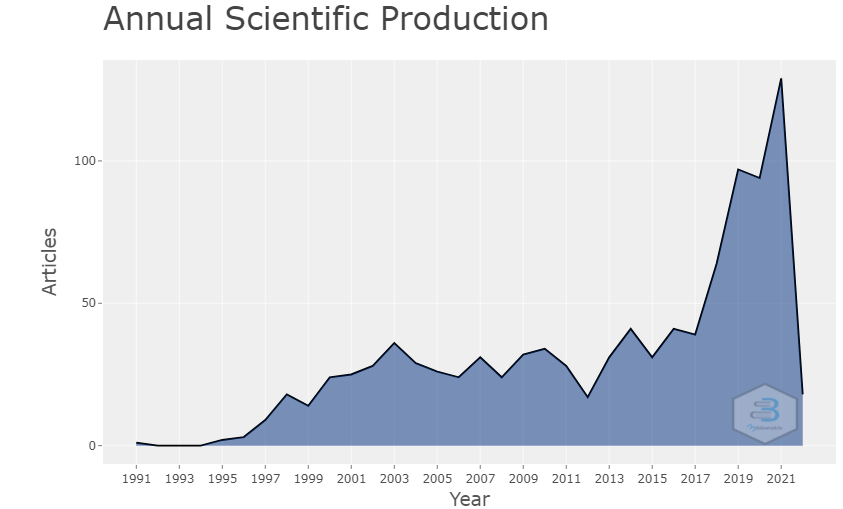
\includegraphics[width=1.0\textwidth]{experiments/Rayxan/PesqBibliogr/ComputacaoQuantica/WoS-20220206/AnnualScientific.png}
    \caption{Evolução da produção científica no \dataset\   Rayxan.}
    \label{fig:evol:anual:Rayxan}
\end{figure}

Observando a figura \ref{fig:evol:anual:Rayxan}, podemos perceber uma evolução gradativa na quantidade de artigos ao longo dos anos, tendo uma explosão de novos artigos a partir do ano de 2015.

\subsection{Evolução das Citações}

\begin{figure}
    \centering
    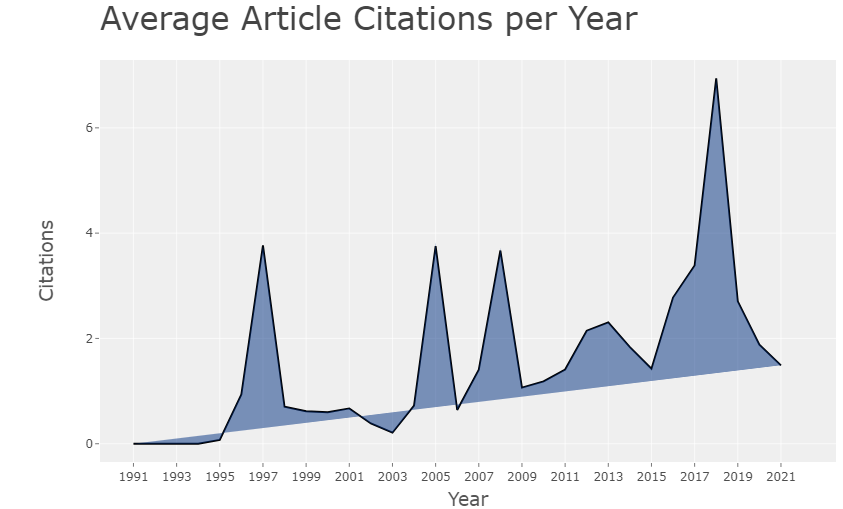
\includegraphics[width=1\textwidth]{experiments/Rayxan/PesqBibliogr/ComputacaoQuantica/WoS-20220206/AverageCitations.png}
    \caption{Evolução das citações ao \dataset\   Rayxan.}
    \label{fig:cit:anual:Rayxan}
\end{figure}

É possível observar em \ref{fig:evol:anual:Rayxan} que o número de citações começou a crescer lentamente a partir de 1991, sofrendo uma explosão neste crescimento em 2015. Se compararmos com a figura \ref{fig:evol:anual:Rayxan} podemos perceber que neste ano, a produção científica também teve um aumento considerável de artigos produzidos, indicando que 2015 foi um ano de extrema importância para a área de estudo da Computação Quântica.

\subsection{Three-Field Plots (Sankey diagram)}

\begin{figure}
    \centering
    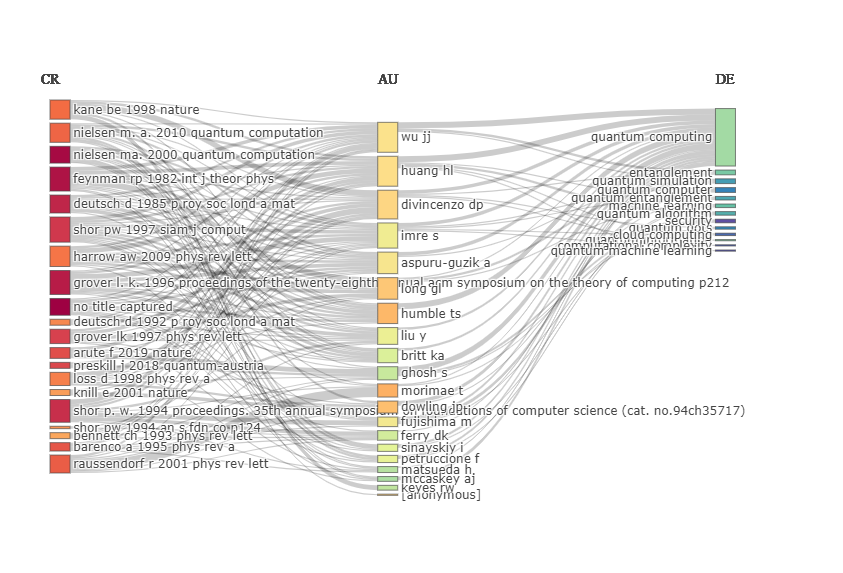
\includegraphics[width=1\textwidth]{experiments/Rayxan/PesqBibliogr/ComputacaoQuantica/WoS-20220206/ThreeFieldsPlot.png}
    \caption{Plotagem ``Três Campos'' (Sankey plot) Rayxan.}
    \label{fig:three:fields:Rayxan}
\end{figure}

A imagem \ref{fig:three:fields:Rayxan} apresenta uma relação entre os autores mais proeminentes (AU), as citações mais frequentes (CR) e por fim, as palavras chaves mais frequentemente usadas (DE). É possível perceber que grande parte dos autores não usou, necessariamente, alguma das palavras chaves apresentadas na imagem, sinalizando que provavelmente os artigos escritos pelos mesmos tratam de assuntos que não condizem com o foco desta análise.




\bibliographystyle{plainnat}
\bibliography{RESIC}

\end{document}.